
\subsection{Cimino, Collins, Baglin 1999 (BESSY)}
\label{sec:Cimino}

This relatively comprehensive paper~\cite{cimino} covers many interesting aspects, among these are:
\begin{itemize}
    \item kinetic energy spectra of photoelectrons,
    \item angular spectra of photoemission,
    \item the dependency of photoelectron yields on photon energy,
    \item total photoemission yields,
    \item and the impact of photon-induced scrubbing on yields and kinetic energies.
\end{itemize}
Many materials used for accelerator technology were studied, among those is Copper but without sawtooth structure.

\subsubsection{Experiment setup}

The source is able to generate monochromatic or broadband synchrotron radiation, which is then guided to the experimental station.
The reflectivity is not measured or taken into account.
This means that the yields correspond to photoelectrons per incident photons $Y$.

\begin{figure}[tbh]
    \centering
    \begin{minipage}[c]{0.65\textwidth}
    	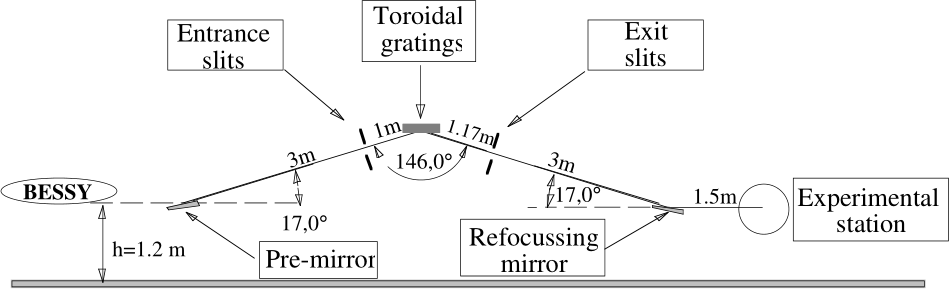
\includegraphics[width=1\textwidth]{../ss/cimino_setup.png}
    \end{minipage}
    \hspace{0.5cm}
    \begin{minipage}[c]{0.30\textwidth}
    	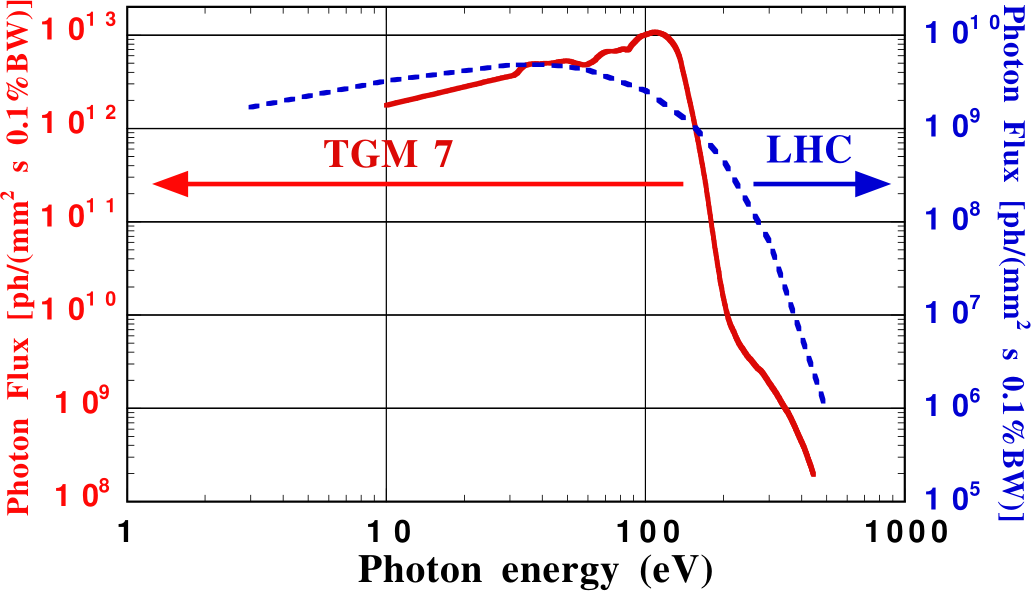
\includegraphics[width=1.0\textwidth]{../ss/cimino_wl_spectrum.png}
    \end{minipage}
    \caption{Left: The experiment setup for the paper presented in Sec.~\ref{sec:Cimino}. Right: The white light spectrum of the SR source.}
    \label{fig:cimino_setup}
\end{figure}


\subsubsection{Results}

The kinetic energy spectra of photoelectrons from Copper were measured before and after scrubbing with white light, see Fig.~\ref{fig:cimino_cu_spectrum}.
It is notable that the photoelectron yields $Y$ are much higher than those presented in Sec.~\ref{sec:Baglin}.
%This can be seen in Tab.~\ref{tab:input_table}, where $Y$ was recovered from the measurement of Sec.~\ref{sec:Baglin} as 2.3$\cdot10^{-2}$, whereas it is around 10 to 6$\cdot10^{-2}$ for as-received and scrubbed samples in this paper.
Regarding the spectra of kinetic energy, it becomes clear that white light scrubbing has a similar effect as surface cleaning with Argon sputtering.
Especially the output of low energy photoelectrons is diminished, meaning that also the total yield decreases significantly.

\begin{figure}[tbh]
    \centering
\end{figure}
\begin{figure}[tbh]
    \centering
    \begin{minipage}[c]{0.47\textwidth}
    	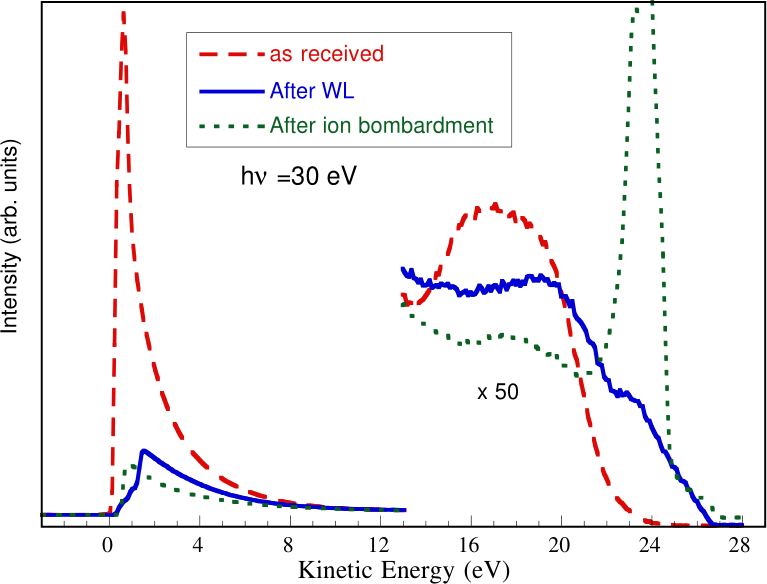
\includegraphics[width=1.0\textwidth]{../ss/cimino_cu_spectrump.png}
    \end{minipage}
    \hspace{0.5cm}
    \begin{minipage}[c]{0.47\textwidth}
        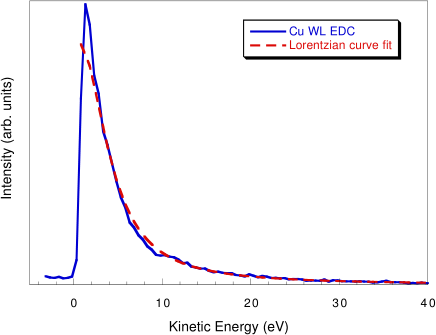
\includegraphics[width=\textwidth]{../ss/cimino_cu_fit.png}
    \end{minipage}
    \begin{minipage}[c]{0.7\textwidth}
        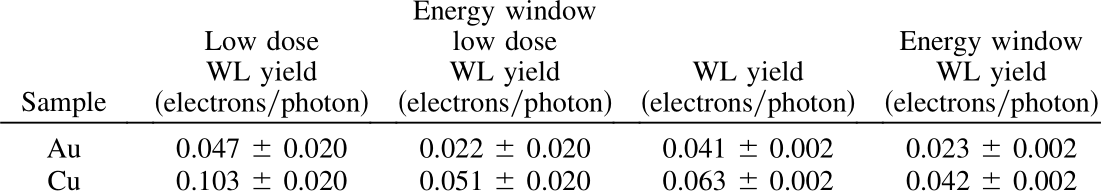
\includegraphics[width=\textwidth]{../ss/cimino_table.png}
    \end{minipage}
    \caption{
        Left: The photoemission spectra for 30~eV photons on Copper (Sec.~\ref{sec:Cimino}).
        The blue curve corresponds to a state after scrubbing has been performed, it is similar to the spectrum after a surface cleaning with ion bombardment.
        \\
        Right: A Lorentzian fit to the low-dose WL spectrum centered at 0.64~eV and 3.7~eV wide.
        \\
        Bottom: WL photoelectron yields for Au and Cu.
        The energy window corresponds to photoelectrons with energies between 1 and 6~eV.
        After WL scrubbing, the yield decreases by about 40\%.
		}
    \label{fig:cimino_cu_spectrum}
\end{figure}

